\chapter[Antecedentes del proyecto]{Antecedentes del proyecto}
\chaptermark{Antecedentes}
\label{ch:antecedentes}

\section{Lenguajes de programación sonora}

La emulación digital de dispositivos analógicos es tan antigua como la misma computación. En concreto, el diseño de programas y lenguajes de programación expresamente destinados a la síntesis sonora tiene sus raíces  en los años 60 del pasado siglo, con lenguajes como \textit{Music 1}, \textit{Music 2}, \textit{Music 3} y \textit{Music 4}, predecesores de \textit{CSound} \cite[~p. xxvii]{Csound_book} que, a pesar de su aspecto primitivo, ha llegado hasta nuestros días y sigue siendo una referencia en el ámbito de la programación sonora. Aunque este lenguaje fue pensado para <<compilar>> los archivos en uno de audio como salida, actualmente es posible usarse en tiempo real gracias al crecimiento del poder de los ordenadores actuales. Precisamente es SuperCollider uno de los  lenguajes que podemos denominar <<modernos>> \cite[~p. ix]{SC_book}, ya que nace para ser ejecutado en tiempo real, además de asimilar herramientas de programación de más alto nivel que \textit{CSound}, como la <<orientación a objetos>>, así como la separación entre lenguaje, intérprete y servidor de sonido, que le confieren una gran versatilidad. 




Existen otros muchos lenguajes pensados para la síntesis sonora, como \textit{Common Music,} \textit{Kyma}, \textit{Nyquist}, and \textit{Patchwork}, entre otros, pero son \textit{CSound} y \textit{SuperCollider} los que han ejercido en mí un gran influjo en la forma de pensar la programación sonora. Algo que no deja de sorprenderme es que estos lenguajes, a pesar de tener un status y coherencia interna propios, usan explícitamente conceptos que provienen de la síntesis analógica realizada con sintetizadores. Sus unidades fundamentales de generación de señal (\textit{Opcode} en \textit{Csound} y \textit{UGen} en \textit{SuperCollider}) utilizan terminología claramente heredada del mundo analógico: \textit{oscilador}, \textit{envolvente}, \textit{filtro}, \textit{control}, \textit{modulación}, etc. Si bien, se introducen otros conceptos que solo pueden ser propios de la síntesis digital por su naturaleza computacional: \textit{tabla de onda}, \textit{aliasing}, \textit{tasa de audio o de control}, etc.

\section{Conectando cables virtuales\dots}

Existen otros sistemas digitales de generación y tratamiento de audio que heredan características propias e interesantes de los sintetizadores modulares y que actualmente tienen una salud de hierro. Me refiero al paradigma de programas como \emph{Pure Data}\footnote{\href{https://puredata.info/}{\texttt{https://puredata.info/}}} o \emph{MAX}\footnote{\href{https://cycling74.com/products/max/}{\texttt{https://cycling74.com/products/max/}}}. No cabe duda que su principal acierto ha sido el de tomar el concepto de \emph{patching} de la síntesis modular como elemento básico de su funcionamiento. Se basan en una interfáz gráfica en la que todo son objetos que el usuario une con cables virtuales a golpe de ratón. A diferencia de los lenguajes de programación basados en texto plano, estos sintetizadores digitales tienen un aspecto visual intuitivo y aún más próximo a lo que significa <<tocar>> un dispositivo analógico. 

\begin{figure}
	\centering
	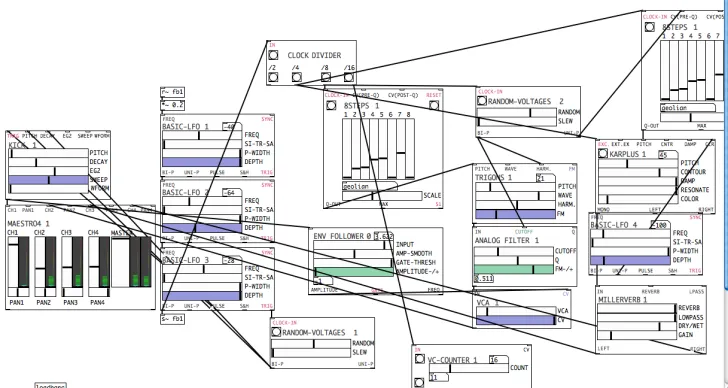
\includegraphics[width=0.7\textwidth]{./puredata_modular}
	\caption[\textit{Patch} en \textit{Pure Data}]{\textit{Patch} de cierta complejidad diseñado en \textit{Pure Data. }}
	\label{fig:puredata_modular}
\end{figure}

Las generaciones más modernas de músicos y artistas sonoros nos hemos educado principalmente con este tipo de software, y nuestro contacto con la síntesis analógica ha sido aprendida a través de estas herramientas, que <<imitan>> el funcionamiento de los viejos sintetizadores.

\section{La era de los \textit{plugins}}
\label{sec:plugins}

Un grupo de programas que han ejercido un influjo más concreto en la creación de \appName~ son los \textit{plugins} de las modernas \textit{DAW} (\textit{Digital Audio Workstation}). Los \textit{plugins} son unidades de generación de señal o de efectos que se aplican arbitrariamente a las pistas de sonido de las <<estaciones de audio digital>>. Típicamente traen una interfaz gráfica que suele imitar con detalle todo tipo de dispositivos analógicos. Existe todo un mercado en torno a estos productos, que vienen a sustituir en muchos casos el uso de aparatos electrónicos, con diseños de una gran fidelidad a los originales. En la interminable lista de \textit{plugins}\footnote{Como muestra, en esta web se encuentran unos 200 \textit{plugins} de libre uso, unos con licencias de código abierto y otros simplemente \textit{freeware}: \href{https://blog.landr.com/best-free-vst-plugins/}{\texttt{https://blog.landr.com/best-free-vst-plugins/}}} que podemos encontrar por la red, tienen un hueco especial aquellos que emulan sintetizadores de todo tipo. 

Existen, por supuesto, emuladores de productos míticos de EMS. Entre los productos de uso libre que podemos encontrar, se puden citar las siguientes emulaciones de EMS Synthi VCS3 y AKS: \textit{Cynthia VST}, \textit{KX-Synth-X16 VST}, \textit{Synthia 2} o \textit{SynthiAKS}, \textit{VCS5}\footnote{Se pueden encontrar listados todos ellos con links de descarga en: \href{https://blog.wavosaur.com/free-ems-vcs3-synthi-aks-vst-emulations/}{\texttt{https://blog.wavosaur.com/free-ems-vcs3-synthi-aks-vst-emulations/}}}. En este punto caben destacar los esfuerzos por ofrecer productos de pago y de alta calidad por empresas como \textit{Ableton} o \textit{Arturia}. Quizás \textit{Arturia Synthi V}\footnote{\href{http://www.futuremusic-es.com/arturia-synthi-v-sinte-plugin/}{\texttt{http://www.futuremusic-es.com/arturia-synthi-v-sinte-plugin/}}} sea el software más completo y elegante del mercado que emula al sintetizador EMS Synthi VCS3.

\begin{figure}
	\centering
	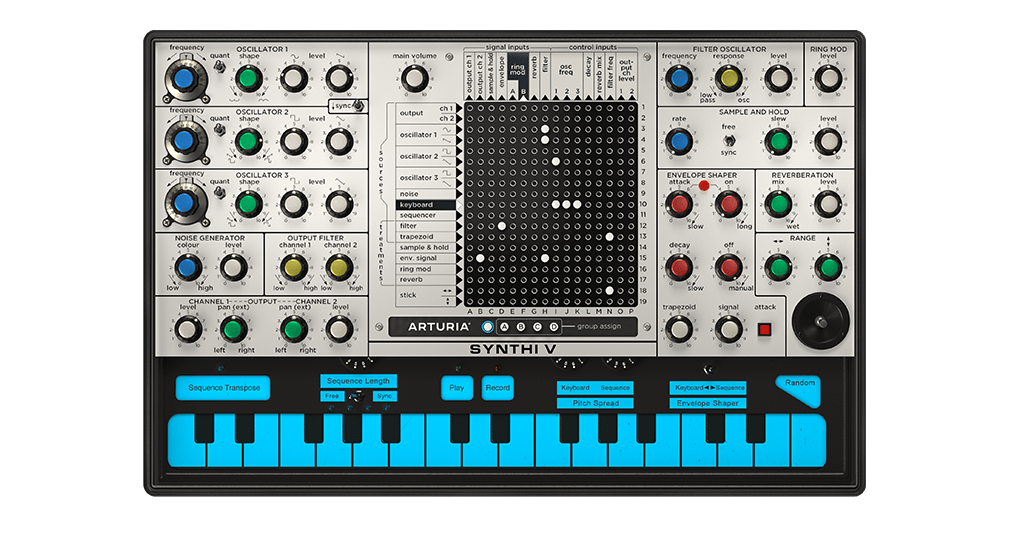
\includegraphics[width=0.7\textwidth]{./synthi_v_arturia}
	\caption[\textit{Arturia Synthi V}]{Aspecto del \textit{plugin} de \textit{Arturia}, \textit{Synthi V}.}
	\label{fig:synthi_v_arturia}
\end{figure}


\section[\appName, ¿un emulador más?]{\appName, ¿un emulador más?}
	\sectionmark{¿un emulador más?}

El proyecto de diseño e implementación de \appName~toma características de distintos productos, ninguno de los cuales abarca todas ellas:

\begin{description}
	\item[Es software libre] \appName~está licenciado bajo los términos de GNU GPLv3. Esto es esencial si no se quiere limitar la información a la que puede acceder el usuario, así como su libertad de modificar y usar el \textit{software}. 
	
	\item[Emula un sintetizador de grandes dimensiones] No es común encontrar un emulador tipo \textit{plugin} con tantos módulos como el Synthi 100. De hecho, sus dimensiones no están exentas de ciertos problemas de manejabilidad y de visionado, que se han intentado resolver de la manera más sencilla y práctica posible.
	
	\item[Emula un sintetizador concreto] Más allá de imitar un modelo concreto de sintetizador, el objetivo está puesto en una unidad concreta, la del Gabinete de Música Electroacústica de Cuenca. 
	
	\item[Tiene un fin pedagógico] Su origen es académico y también su destino. La elaboración de este trabajo ha coincidido con la restauración del Synthi 100 del GME de Cuenca, de forma que este \textit{software} ha sido pensado para ser utilizado tanto para la difusión y formación en torno al GME en la Universidad de Cuenca, como para la educación en general. 
	
	\item[Está escrito en lenguaje de SuperCollider] \textit{sclang} es un lenguaje diseñado expresamente para SuperCollider, lleno de características de propósito general que facilitan la escritura de \textit{scripts} para el diseño de audio. El hecho de ser software libre, su simplicidad y su  compilación \textit{just in time} lo hacen apto para \textit{live coding} y para la creación de programas realmente complejos, como el caso de \appName. La elección de este lenguaje está muy unida a su destino pedagógico.
\end{description}



